\documentclass{article}
\usepackage{blindtext}
\usepackage[margin=0.75in]{geometry}
\usepackage[utf8]{inputenc}
\usepackage{amsmath}
\usepackage{stackengine}
\usepackage[pdftex]{graphicx}
\usepackage{float}
\usepackage{newlfont}
\usepackage{amssymb}
\usepackage{verbatim} 
\usepackage[final]{pdfpages}
\usepackage{setspace}
\setlength{\parindent}{0pt}

\title{Multi-Armed Bandit Problem}
\author{Sunith Suresh, Lin Xiao, Ilan Man and Sanjay Hariharan}
\date{\today} 
\begin{document}
\maketitle

\section{Introduction}

This paper explores the multi-armed bandit problem (MAB). A multi-armed bandit is a sequential experiment with the goal of achieving the largest possible reward from a payoff distribution with unknown parameters. The term multi-armed bandit comes from slot machines where each machine is known as a one-armed bandit. In this set up, at each iteration the player must decide which arm of the experiment to observe next.\\

The task is complicated by the stochastic nature of the bandits in the following two ways:

\begin{enumerate}
\item A suboptimal bandit can return many winnings, purely by chance, which would make us believe that it is a very profitable bandit. Similarly, the best bandit might not yield a reward if only played a few times.
\item If we have found a bandit that returns good results, do we keep drawing from it to maintain our good score, or do we try other bandits in hopes of finding an even better bandit? How do we know when to switch and when to stick to the current bandit? This is known as the \textit{exploration vs. exploitation} dilemma.
\end{enumerate}

This is a classic reinforcement learning problem in machine learning literature, as well as a game theoritic problem in economic theory.\\

This paper reviews several strategies for selecting machines, including a creative application of dynamic programming. Note that there are many variations on the stochastic MAB, including contextual bandit and adverserial bandit, which we will not discuss here and is outside of the scope of this paper. 

\section{Multi-armed Bandits}

In machine learning literature, the stochastic multi-armed bandit problem is formulated as:

\begin{quote}
Given $K$ machines, each with an unknown probability of yielding a reward, which come from a fixed but unknown distribution parameterized by $\theta_i$, for $i \in (1, ..., K)$, and $N$ total plays, decide which machines to play in order to maximize the total reward.
\end{quote}

\subsection{Reget vs. Reward}

It is common in the literature to express the maximum reward as minimzing \textit{regret} compared to the best arm in hindsight, acting as a sort of opportunity cost. That is, define regret at each step as $r_{t} = R^*_{t} - R_{t,i}$, where $R^*$ is the reward yielded by selecting the best machine and $R_{t,i}$ is the reward yielded by selecting machine $i$ at time $t$. Note that in reality we don't know what the best machine is - this formulation is purely a way to compare the performance of algorithms with simulated data. The goal is then to devise a strategy to minimize $\sum_{t=1}^N r_{t}$. Note that since this is a stochastic problem, we aim to minimize regret in expectation or with high probability.\\

\subsection{Exploitation vs. Exploration}

The tension between playing all the machines many times and only playing the best machine is a key concern for optimizing an algorithm. The problem with exploring too much is that every time you play a machine that isn't the best, you incur some regret, since you won't be playing a machine with highest expected reward. In addition, if you view machines as, for example, websites that users click on, then every time you send users to a bad website, you risk losing them forever, if they have a very unfavorable experience. On the other hand, if you exploit too quickly, then you won't have explored the space of possible machines and may miss out on the most optimal machine. This could be very costly, especially if you don't change your mind later on - you will always incur some cost in the form of the regret function.\\

\section{Bayesian approaches: Bernoulli Bandit}

A popular approach to solving the MAB problem is to minimize regret using Bayesian inference. Specifically, assume that rewards are distributed as a Bernoulli with some latent parameter, $\theta_i$, specific to each machine. In addition, we can put a prior distribution on $\theta_i$ and update our belief about it as we run the algorithm and learn which machines are better than others. Since rewards are generated from a Bernoulli distribution, a natural choice for the distribution on $\theta_i$ is a Beta. Formally stated:

$$\theta_i \sim \text{Beta}(\alpha_i, \beta_i)$$
$$r_i = \text{Reward from machine i} \sim \text{Bernoulli}(\theta_i)$$

Exploiting the conjugacy of the Beta-Bernoulli model, the posterior distribution of getting a reward from $\text{machine}_i$, after playing for $N$ iterations is:
$$\text{Beta}(\alpha_i + R_{N}, \beta_i + T - R_{N})$$

where $R_{N} = \sum_{t=1}^{N}r_{t}$.\\

Before beginning to play, we assume no prior knowledge about any machine's propensity to yield a positive reward. Therefore, we initially set $\alpha_i, \beta_i = 1$, which is a common objective prior for the Beta distribution.\\

\subsection{Dynamic Programming}

As mentioned above, our goal is to either minimize regret or maximize total expected rewards, $\mathbb{E}(R_N)$. Under the above setup, we constructed an approach to maximizing future expected rewards based on a backwards, dynamic programming scheme. Note that we derive the algorithm assuming $K = 2$ machines.\\

Before we discuss how to construct our acquisition function $U(\theta|X)$ which will help us decide which machine to play at each iteration, we note the following interesting observations:

\begin{enumerate}
\item At time $T = 1$, we have no prior belief concerning any machine. Thus, it will not matter which machine we pick the first time around, though it will influence all subsequent choices.
\item At time $T = N$, we are at our final trial, and thus are only concerned with the reward on this trial. As such, we opt for a \textbf{greedy} approach and pick the machine with the highest expected reward. Using a Beta posterior, that is:  $\underset{i}{\text{argmax}}(\frac{\alpha_1}{\alpha_1 + \beta_1}, \frac{\alpha_2}{\alpha_2 + \beta_2}$)
\item For times $T = 2, ..., N-1$, we must choose the machine based on the expected sum of future rewards, based on our framework above: $\mathbb{E}(\displaystyle\sum_{i=1}^{N} r_i)$
\item In general, at time $T = t$, $\mathbb{E}(\displaystyle\sum_{i=t}^{N} R_i|M_{1:t-1}, R_{1:t-1})$ = $\mathbb{E}(\displaystyle\sum_{i=t+1}^{N} R_i|\theta)$ + $\mathbb{E}(R_t|\theta)$ 
	\begin{itemize}
	\item $M_{1:t}$ = machines chosen from times $1, ..., t$ 
	\item $R_{1:t}$ = rewards given from times $1, ..., t$
	\end{itemize}
\end{enumerate}

Given we perform $N$ trials, we construct our algorithm in a backwards fashion:

\begin{enumerate}
\item For $T = N$:
	\begin{itemize}
	\item For each node, we choose the greedy, i.e. the one with the maximum expected reward.
	\end{itemize}
\item For $T = N-1$:
	\begin{itemize}
	\item Given that we know the most optimal choice for the last trial, we select the machine on this trial that will give us the maximum expected sum of future rewards
	\item $\mathbb{E}(R_{N-1} + R_{N})$, and we know $R_N$ from the previous iteration
	\end{itemize}
\item For $T = N-2,..., 2$:
	\begin{itemize}
	\item We follow similar intuition as above, choosing the most optimal choice for the maximum expected sum of future rewards, given the optimal choice for all subseqent trials already calculated
	\item $\mathbb{E}(\displaystyle\sum_{i=T}^{N} R_i)$ = $\mathbb{E}(\displaystyle\sum_{i=t+1}^{N} R_i)$ + $\mathbb{E}(R_t)$
	\end{itemize}
\item For $T = 1$:
	\begin{itemize}
	\item As mentioned above since the first iteration will not influence our decision, as we have no prior knowledge, we select any machine at random.
	\end{itemize}
\end{enumerate}

As an illustration, consider the following tree. Here we denote $f(\alpha_1, \beta_1, \alpha_2, \beta_2)$ as the posterior parameters of the machine at time $T$, starting from the beginning \textbf{CAN YOU ELABORATE ON WHAT f IS? WHAT'S THE OUTPUT? WHAT ARE THE BRANCHES EXACTLY?}:

\begin{figure}[H]
\centering
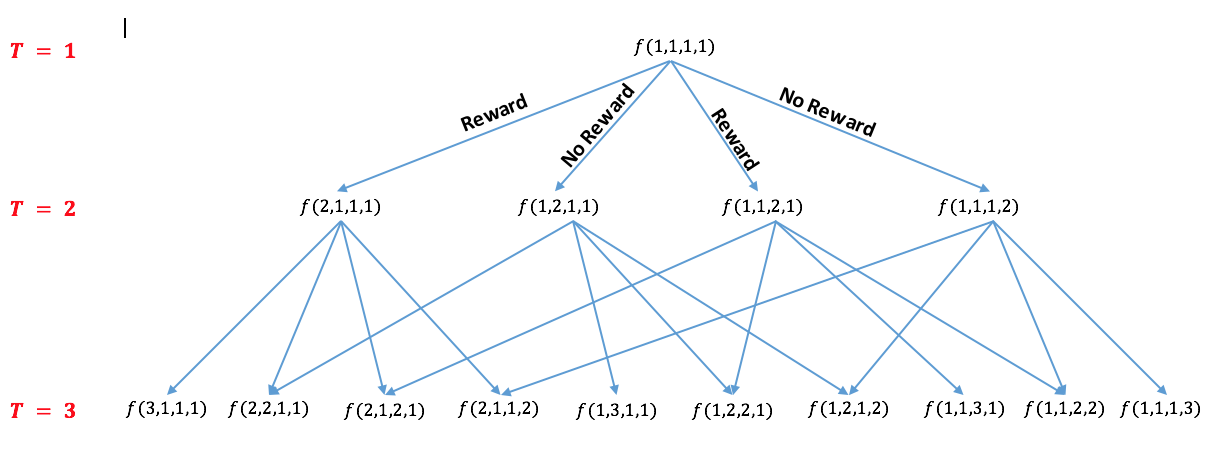
\includegraphics[scale=0.75]{Dynamic_Programming_Tree.png}
\caption{Forest of Possible Outcomes}
\end{figure}

As time increases, the complexity of possible branches increase exponentially, but it is important to note that some branches merge back together. Visually, our algorithm takes in two pieces of information:

\begin{enumerate}
\item Current parameters of the machine based on previous observations
\item Number of Trials we expect to perform
\end{enumerate}

Our algorithm creates a tree of all possible future states, like above, and dynamically works backwards, assuming at the final stage we want to be completely greedy (since it is our last trial). The output of the algorithm is \textbf{the specific machine we should play at the current stage}, as well as the expected sum of rewards given you follow the algorithm at each trial.\\

One might assume that we would be greedy at every approach, but our algorithm proves otherwise. It bases its decision on expected future rewards, and it is interesting to see it choose the machine with the lower expected reward, based on its future possible states.\textbf{WHERE HAVE WE SEEN THIS? DO YOU HAVE AN EXAMPLE? ALSO WHY IS IT INTERESTING? I.E. BECAUSE WE WOULDN'T EXPECT IT BASED ON THE GREEDY APPROACH? MAYBE TALK ABOUT WHY WE DIDN'T IMPLEMENT THIS? AND CAN YOU ADD IN SOMETHING LEADING TO THE NEXT SECTIONS WHERE WE DISCUSS OTHER ALGORITHMS THAT WE IMPLEMENTED?}

\subsection{Thompson Sampling}

As mentioned in the algorithm above, our approach to solving the MAB problem is inherently Bayesian. Below we outline a popular approach used in practice called Thompson Sampling, which relies on Bayesian mechanics. The general algorithm is as follows:

\begin{enumerate}
\item For $t = 1, ..., N$
	\begin{enumerate}
	\item $U(\alpha_i$, $\beta_i) = i$  // select machine $i$ at time $t$ using the acquisition function
	\item $r_t \sim \text{Bernoulli}(\theta_{i})$   // We play machine $i$, and observe reward $r_t$
	\begin{itemize}
		\item If $r_t = 1: \alpha_i = \alpha_i + 1$   // increase our positive belief in machine $i$
		\item else if $r_t = 0: \beta_i = \beta_i + 1$  // increase our negative belief (i.e. failure) in machine $i$
	\end{itemize}
	\item $R_t = R_t + r_t$		// add reward at time $t$ to running total
	\end{enumerate}
\end{enumerate}

This algorithm provides a framework for how to think about this problem in a Bayesian way. To maximize expected rewards, we must optimally choose the policy function $U$.\\

Below we review 3 ways to select the policy, $U$:

\begin{enumerate}
\item \textbf{Explore}: Randomly select one of the $K$ machines, without considering how many win/losses we've seen. This is a pure exploratory strategy and is used for comparison purposes only. In reality no one would choose this approach.
\item \textbf{Exploit}: Sample each $\theta_i \sim Beta(\alpha_i, \beta_i)$. Select $\underset{i}{\text{argmax}}\text{ }\mathbb{E}[\theta_i]$. This is called exploit because we are greedily choosing the best machine at each step based on expected rewards. Note however that even if we select the best expected machine, there is a probability of $\frac{\beta_i}{\alpha_i + \beta_i}$ that it fails to generate a reward. So the amount of exploration is much less than above but still non-zero. That this approach is known as \textit{Adbandit}.
\item \textbf{Thompson-Sampling}: Sample each $\theta_i \sim Beta(\alpha_i, \beta_i)$. Select $\underset{i}{\text{argmax}}\text{ }\theta_i$. This approach falls somewhere between Exploit and Explore, but is much closer to Exploit. In expectation we expect Thompson-Sampling to be very close to Exploit.
\end{enumerate}

We ran these three approaches on a dataset of $K=5$ machines with true reward distribution, $[0.05,0.1,0.3,0.2,0.5]$ and calculate the cumulative regret after 300 iterations. Below is the output for 1 particular run:

\begin{figure}[H]
\centering
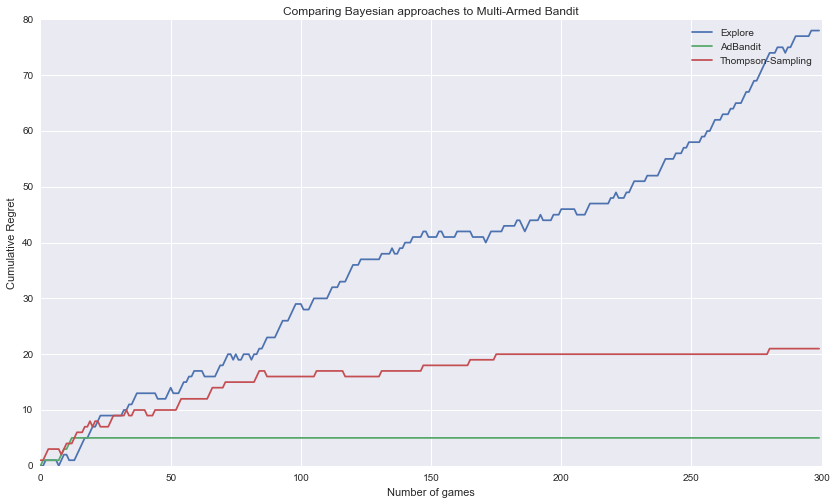
\includegraphics[scale=0.4]{thompson_regret.png}
\caption{Cumulative Regret}
\end{figure}

As expected, the Explore strategy performs the worst. In this run, Adbandit performed the best. If we took the average of many runs, we'd expect Thompson-Sampling and Adbandit to perform similarly. Note that Adbandit finds the best machine very quickly and stays there. If $K$ was larger, then it would be more exploring, or potentially get stuck in a poorly performing machine for a long time before finding a better one. We expect Thompson-Sampling to outperform Adbandit for larger $K$.

\subsection{$\epsilon$-greedy}

The most simple approach to tackling the MAB problem is the $\epsilon$-greedy algorithm. As explained earlier, the greedy algorithm always takes the best action at every trial. In other words, it simply chooses the bandit with highest expected reward at every iteration. The problem with this purely exploitative approach is that, it will take a large number of iteration to explore all the machines and converge onto the best machine. The $\epsilon$-greedy algorithm is almost a greedy algorithm as it generally exploits the best machine, however every once in a while it explores other machines.\\ 

The parameter $\epsilon$ controls the percentage of iterations for which the algorithm explores machines. The algorithm can be described as follows: For a proportion $1 - \epsilon$ of the trials, choose the best machine(i.e the machine with highest expected reward), and for a proportion of $\epsilon$ explore other machines (with uniform probability).\\

Given machines $\{1,...,K\}$ with initial empirical means $\{\hat{\mu_1(0)},...,\hat{\mu_K(0)}\}$ For trials $t = \{1,...,N\}$, the probability of choosing machine $i$ is given by

$$p_i(t+1) = \begin{cases}
  1- \epsilon + \frac{\epsilon}{K}, & \text{if } i = argmax_{j=1,..,K}\hat{\mu_j(t)}, \\
  \frac{\epsilon}{K}, & \text{otherwise}.
\end{cases}$$


It follows from the algorithm that if $\epsilon = 0$, the algorithm reduces to a purely exploitative one, whereas if $\epsilon = 1$, it reduces to a purely explorative one. Therefore the value of $\epsilon$, defined by the user, controls the level of exploration and exploitation employed by the algorithm.\\

The $\epsilon$-greedy algorithm is considered to be suboptimal due to the constant value of $\epsilon$. As the number of trials increase, asymptotically we can be reasonably certain as to which machine is the best machine from the observed rewards. However, the algorithm will always explore for $\epsilon$ percent of the trials. To address this issue, variants of the algorithm have been proposed. Two popular variants are known as $\epsilon$-first algorithm and $\epsilon$-decreasing algorithm.\\

The $\epsilon$-first algorithm consists of doing the exploration all at once at the beginning and then switching to pure exploitation. Given $N$ total trials, for $\epsilon N$ trials, the machines are randomly chosen (with uniform probability). After the exploration phase, for the remaing $\big( 1-\epsilon \big) N$ trials, the algorithm switches to pure exploitation, choosing the machine with highest expected rewards.\\

The $\epsilon$-decreasing algorithm consists of decreasing the value of $\epsilon$ with number of trials. The algorithm progresses from highly explorative approach in the beginning to a highly exploitative one towards the end.\\

CesaBianchi and Fisher (1998) found that $\epsilon$-decreasing algorithm is theoretically efficient (with respect to regret). However empirical studies by Vermorel and Mohri (2005) do not seem to find any significant improvements with the variants of the algorithm when compared to the original $\epsilon$-greedy algorithm.\\

\begin{figure}[H]
\centering
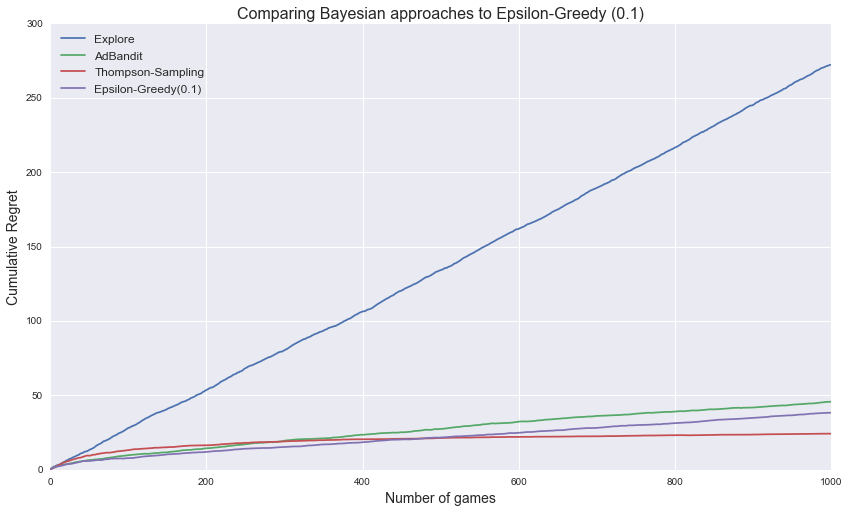
\includegraphics[scale=0.4]{eps_greedy.png}
\caption{Cumulative Regret}
\end{figure}

References
Bandit algorithms for Website Optimization by J. White
algorithms for the multi-armed bandit problem by V. Kuleshov and D. Precup
Multi-armed Bandit algorithms and Empirical Evaluation M. Mohri and J. Vermorel
Peter Auer, Nicolo Cesa-Bianchi, and Paul Fischer. Finite-time analysis of the multiarmed bandit problem. machine Learning, 47((2-3)), 2002.

\subsection{Upper Confidence Bounds}

The other algorithms presented in this paper are similar in that they pay attention only to how much reward they’ve gotten from the machines. This means that they're likely to under-explore options whose initial experiences were not rewarding, even though they may not have enough data to be confident about those arms. One naive approach to solving this problem is to run the algorithm multiple times and take the average of the results. Another could be to run the algorithm for a very long time and hope the probabilistic nature will eventually correct for random variation in the reward distribution. Another approach is to use probability theory to bound our confidence in how good or bad each machine is. This is exactly what Upper Confidence Bounds does.\\

The upper confidence bound (UCB) family of algorithms selects the machine with the largest upper confidence bound at each round. This paper will only focus on UCB1, but note that there are many variants of the UCB family. The more times you play a machine, the tighter the confidence bounds become. So as the number of plays for each machine increases, the uncertainty decreases, and so does the width of the confidence bound.\\

We want to know with high probability that the true expected payoff of a play $\hat{\mu_i}$ is less than our prescribed upper bound:

$$\bar{\mu_{i}} + \sqrt{\frac{2 ln (t)}{n_i}}$$

Where $\bar{\mu_{i}}$ is the average reward obtained from machine $i$ and $n_i$ is the number of times machine $i$ has been played so far.\\

This upper bound is the sum of two terms, where:

\begin{enumerate}
\item the first term is the average reward
\item the second term is related to the one-sided confidence interval for the average reward according to the Chernoff-Hoeffding bounds
\end{enumerate}

Recall that since rewards follow a Bernoulli distribution, we can apply Chernoff-Hoeffding to upper bound the probability that the sum of rewards from each machine deviates from its expected value:

$$\displaystyle \textup{P}(Y + a < \mu) \leq e^{-2na^2}$$

This confidence bound grows with the total number of actions we have taken but shrinks with the number of times we have tried this particular action. This ensures each action is tried infinitely often but still balances exploration and exploitation. It can be shown that the regret for UCB1 grows with \textbf{ln n}, as witnessed below for the optimal machine.\\

Note that in addition to keeping track of our confidence in the estimated values of each machine, the UCB algorithm doesn’t use randomness at all. Unlike the other algorithms in this paper (and in the literature) it’s possible to know exactly how UCB will behave in any given situation. This can make it easier to reason about at times.

\subsubsection{UCB1: algorithm}

Assuming $K$ machines:

\begin{enumerate}
\item Play each arm once
\item Observe rewards $r_i$, for $i = 1, ..., K$
\item Set $n_i = 1$, for $i = 1, ..., K$
\item set $\bar{\mu_{i}} = \frac{r_i}{n_i}$
\item For time $t = K+1, ..., N$:
	\begin{enumerate}
		\item Play arm $\hat{i} = \underset{i}{\text{argmax}}\text{ }(\hat{\mu_{i}} + \sqrt{\frac{2 ln (t)}{n_i}})$
		\item Observe reward $r$
		\item $r_{\hat{i}} = r_{\hat{i}} + r$
		\item $n_{\hat{i}} = n_{\hat{i}} + 1$
		\item update $\hat{\mu_{i}} = \frac{r_{\hat{i}}}{n_{\hat{i}}}$
	\end{enumerate}
\end{enumerate}

Below we run UCB1 on the same dataset as above:

\begin{figure}[H]
\centering
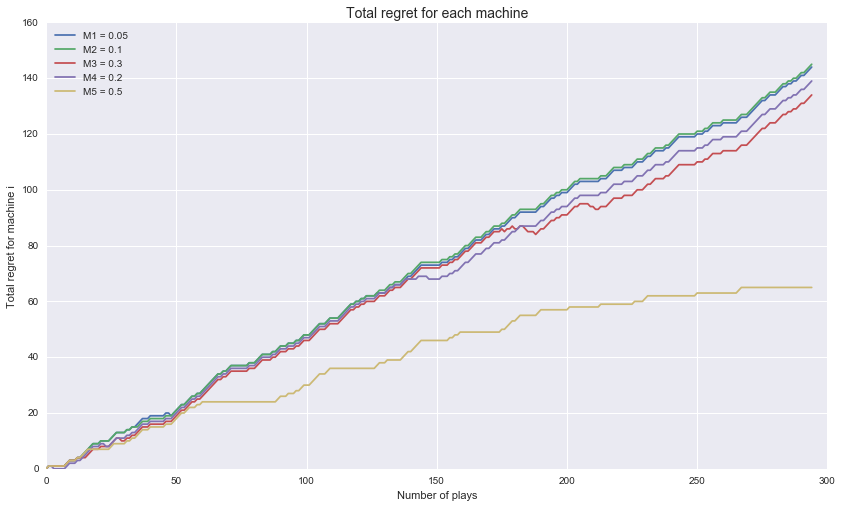
\includegraphics[scale=0.4]{UCB_regret.png}
\caption{Cumulative for all 5 machines}
\end{figure}

Above we see that, as expected, Machine 5 has the lowest regret, since it has the highest $\theta$. 

\begin{figure}[H]
\centering
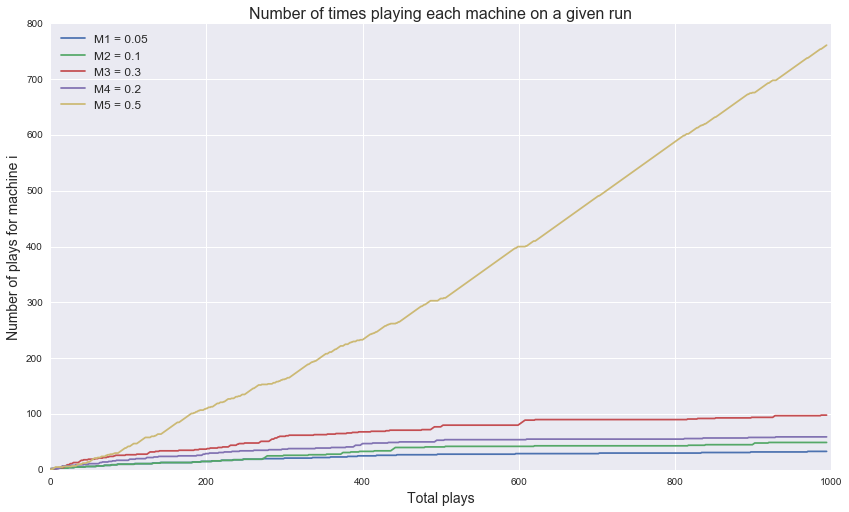
\includegraphics[scale=0.4]{UCB_num_plays.png}
\caption{Switching between machines}
\end{figure}

As expected, machine 5 is played the most often, even though the worse off machines are still being played. Separation from the other machines occurs around 60 iterations. Also note that even at 300 runs, there isn't much separation between machines 1 and 2, given how similar their $\theta$ is.

\begin{figure}[H]
\centering
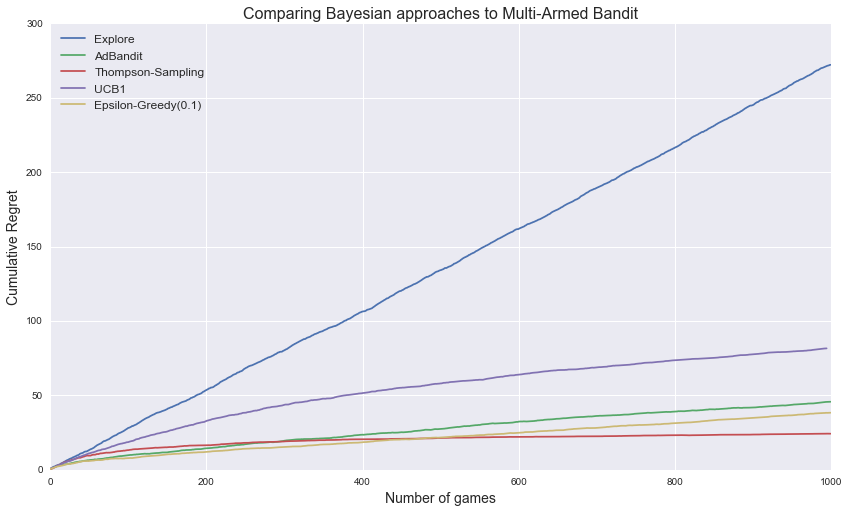
\includegraphics[scale=0.4]{all.png}
\caption{Comparing all 5 approaches}
\end{figure}

UCB1 does the worst in this particular run, compared to the other non-naive approaches. This suggests that while it provides nice theoretical guarantees, Bayesian heuristic approaches and even simple ones like $\epsilon$-greedy can outperform it.

\subsection{Gaussian Process and Reinforcement Learning}

- Lin
\begin{itemize}
\item assume knowledge of GPs, so no need to explain what a GP is
\item quick overview of how MAB relates to reinforcement learning
\item quick overview of how GPs relate to reinforcement learning
\item using the mechanics of GP, what the connection between GP and MAB is
\item show a chart or two like in the presentation
\item this will be multiple sections
\end{itemize}

\section{Conclusion}

\section{References}


\end{document}
